%%%%%%%%%%%%%%%%%%%%%%%%%%%%%%%%%%%%%%%%%%%%%%%%%%%%%%%%%%%%%%%%%%%%%%%%%%%%%%%%
%%
%%   BornAgain User Manual
%%
%%   homepage:   http://www.bornagainproject.org
%%
%%   copyright:  Forschungszentrum Jülich GmbH 2016
%%
%%   license:    Creative Commons CC-BY-SA
%%
%%   authors:    Scientific Computing Group at MLZ Garching
%%               M. Ganeva, G. Pospelov, W. Van Herck, J. Wuttke
%%
%%%%%%%%%%%%%%%%%%%%%%%%%%%%%%%%%%%%%%%%%%%%%%%%%%%%%%%%%%%%%%%%%%%%%%%%%%%%%%%%

\part{Usage}\label{PUSE}

\chapter{The three interfaces of \BornAgain}  \label{sec:API3}

%%%%%%%%%%%%%%%%%%%%%%%%%%%%%%%%%%%%%%%%%%%%%%%%%%%%%%%%%%%%%%%%%%%%%%%%%%%%%%%%
\section{Architectural overview}
%%%%%%%%%%%%%%%%%%%%%%%%%%%%%%%%%%%%%%%%%%%%%%%%%%%%%%%%%%%%%%%%%%%%%%%%%%%%%%%%

The overall architecture of \BornAgain\ is outlined in \cref{Farch1}.
The core of \BornAgain\
\index{Core|see {\Code{libBornAgainCore}}}
comprises functionality to construct arbitrary hierarchical sample models,
to setup instrument models,
and to compute the expected detector image for any given sample and instrument model.
Furthermore \BornAgain\ comes with various minimizers that optimize model parameters
to fit the simulated detector image to a given experimental image.
All this functionality is implemented in a library, \Code{libBornAgainCore}.

\begin{figure}[tbh]
\begin{center}
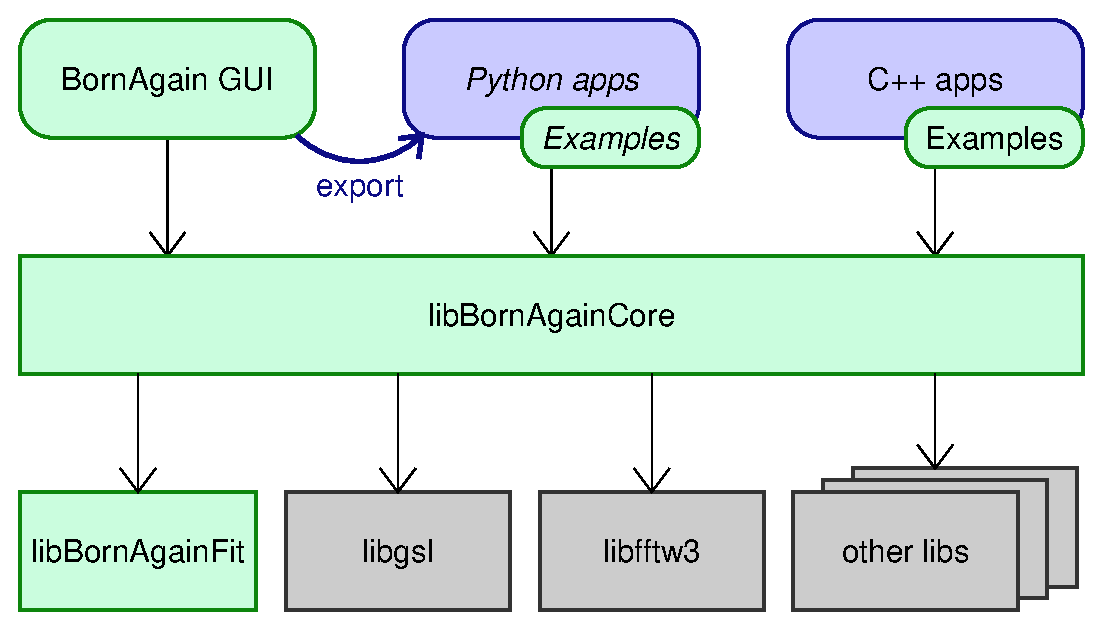
\includegraphics[width=0.7\textwidth]{fig/drawing/architecture1.ps}
\end{center}
\caption{Overall architecture of \BornAgain.
\index{Architecture!applications and libraries}%
Applications are shown as oval fields, libraries as rectangles.
Black arrows indicate ``depends on''.
Green fields designate software that is part of \BornAgain.
Gray fields are external dependences
(only two external libraries are explicitly shown;
several more are listed in the online compilation instructions).
Blue fields indicate stand-alone applications that use \BornAgain's
two Application Programming Interfaces (the C$++$ API and the Python API).
\index{C++!using BornAgain from}
\index{Python!using BornAgain from}
\index{Application Programming Interface}
While such applications are to be written by users,
some examples come with the \BornAgain\ source distribution,
and are explained in the following Manual chapters.
It is also possible to export a simulation setup from GUI as Python code.
The binding of C++ to Python is highly simplified here.
For a more accurate picture, see \Cref{FarchPy}.}
\label{Farch1}
\end{figure}

\index{libBornAgainCore@\Code{libBornAgainCore}}
This library, in turn, depends on a number of other libraries.
One of these, the minimizer wrapper \Code{libBornAgainFit}
\index{libBornAgainFit@\Code{libBornAgainFit}}
\index{Minimizers|see \Code{libBornAgainFit}}
has been written specifically for use in \BornAgain,
and for the time being is only distributed as part of \BornAgain,
though in the future it may find applications in other contexts.
The other library dependences of \Code{libBornAgainCore}
are multi-purpose libraries that are easily available as open-source packages.
\index{Dependences!libraries}

The library \Code{libBornAgainCore} can be used in three different ways:
From its graphical user interface (GUI), or
from user-written stand-alone applications in the programming languages C$++$ or Python.
These different approaches are briefly outlined below.
The Python interface is then described at length in the next chapters.

%%%%%%%%%%%%%%%%%%%%%%%%%%%%%%%%%%%%%%%%%%%%%%%%%%%%%%%%%%%%%%%%%%%%%%%%%%%%%%%%
\section{Using \BornAgain\ from its Graphical User Interface}
%%%%%%%%%%%%%%%%%%%%%%%%%%%%%%%%%%%%%%%%%%%%%%%%%%%%%%%%%%%%%%%%%%%%%%%%%%%%%%%%
\index{Graphical User Interface|(}
\index{bornagain@\Code{bornagain}|see {Graphical User Interface}}
\index{Exectutable!bornagain@\Code{bornagain}|see {Graphical User Interface}}
\index{Binary|see {Executable}}
%\index{Project name!BornAgain@\BornAgain}

The project \BornAgain\ comes with a stand-alone application called \Code{bornagain}
that provides a Graphical User Interface (GUI).
Note that we distinguish between the GUI executable \Code{bornagain},
the underlying library \Code{libBornAgainCore}, and the project \BornAgain\ at large.

The GUI allows users to quickly setup a simulation, to visualize simulated
detector images, to compare with experimental images, and to run fits.
It provides comfortable access to much, but not all the functionality
of \Code{libBornAgainCore}.
Depending on application fields,
users may sooner or later reach the limits of current GUI support.
Other users may have repetitive tasks that are cumbersome under a GUI.
In such cases, users can export their sample and instrument models from
the GUI as a Python script,
and continue work by directly editing the Python code.
\index{Export!Python from GUI}

\Link{Documentation of the GUI is available online:\\
      \url{http://www.bornagainproject.org/documentation/usage/gui}}
\index{Graphical User Interface|)}

%%%%%%%%%%%%%%%%%%%%%%%%%%%%%%%%%%%%%%%%%%%%%%%%%%%%%%%%%%%%%%%%%%%%%%%%%%%%%%%%
\section{Using \BornAgain\ from Python}
%%%%%%%%%%%%%%%%%%%%%%%%%%%%%%%%%%%%%%%%%%%%%%%%%%%%%%%%%%%%%%%%%%%%%%%%%%%%%%%%
\index{Python!using BornAgain from|(}
\index{Application Programming Interface!Python|(}

\BornAgain\ simulations and fits can be set up and run from Python programs
or from a Python command-line interpreter like \Code{IPython}.
\index{IPython}
\index{Command line!Python}
A short program in an interpreted language like Python is customarily called
\index{Script!Python}
\index{Python!script}
a \E{script},
and therefore in the following we will talk about \E{Python scripts}.
Of course this does not preclude the possibility that such scripts evolve into
complex programs, modules, or packages.
And anything we say about scripts also applies to usage of \BornAgain\ in an
interactive Python session.%
\index{Interactive!Python session}%
\index{Python!interactive use}%

Usage of \BornAgain\ in a Python script should start with the command
\setPy
\begin{lstlisting}
import bornagain as ba @\label{import_as}\index{Import!\BornAgain\ to Python|(}@
\end{lstlisting}
This then allows calls to \BornAgain\ in commands like
\pagebreak[2]
\begin{lstlisting}[language=python, style=eclipseboxed,name=ex1,nolol]
air = ba.HomogeneousMaterial("Air", 0.0, 0.0) @\label{constructor_beg}@
air_layer = ba.Layer(air)
sample = ba.MultiLayer() @\label{constructor_end}@
sample.addLayer(air_layer) @\label{class_func_call}@
\end{lstlisting}
The function calls in lines \ref{constructor_beg}--\ref{constructor_end}
return new \E{objects}.
\index{Object!constructor}
These objects are instances of \E{classes} defined in \BornAgain.
\index{Class!Instantiation}
In the language of object-oriented programming,
a Function that returns a new instance of a class is called a \E{constructor}.
\index{Constructor}
In Python, as in C++, constructor names coincide with class names;
so the constructor function \Code{Layer(material)} will return an
object of class type \Code{Layer}.

\begin{figure}[tb]
\begin{center}
\includegraphics[width=0.72\textwidth]{fig/drawing/architecturePy.ps}
\end{center}
\caption{Relation between the BornAgain C++ libraries and the Python layer.
\index{Architecture!Python binding}%
Python code is indicated by \textsl{slanted font}.
Colors as in \Cref{Farch1}.
Bold arrows indicate ``depends on'' for code that is automatically generated
by the software tool Swig.%
\index{Swig}%
\index{Python!Swig}%
}
\label{FarchPy}
\end{figure}

To prevent accidental use of class or constructor names,
they are encapsulated in a \E{namespace}
\index{Namespace}
called \Code{bornagain}.
The \Code{import} command in the above code line~\ref{import_as}
makes this namespace available under the shortcut \Code{ba}.
\index{Import!\BornAgain\ to Python|)}
Note, however, that not all calls to \BornAgain\ require
(and can be recognized by) the prefix \Code{ba}.
The function call \Code{addLayer} in line~\ref{class_func_call}
is defined inside the \BornAgain\ class \Code{MultiLayer}.
The programmer is supposed to know that \Code{sample} is an instance of
class \Code{MultiLayer}, which is part of \BornAgain.
Therefore, there is no need (and no way) to adorn function calls like \Code{addLayer}
with the namespace label \Code{ba}.

The entirety of classes and functions provided by \BornAgain\
and exposed to Python forms the \E{BornAgain Python API}.
An API (Application Programming Interface)
\index{Application Programming Interface!Python}
is a kind of protocol that tells a programmer how to use a library.
In this perspective, the research scientist
who uses Python to set up simulations or fits
is seen as a \E{programmer} who writes an application program.
This notwithstanding, he is still a \E{user}
of the BornAgain Python library.
The relation of this library to the underlaying C++ library is explained
in \Cref{FarchPy}.

The remaining chapters of this \Cref{PUSE} of the BornAgain Manual
contain tutorial examples how to use the BornAgain Python API.
\index{Tutorial}
\Cref{PREF} provides an incomplete reference.
\index{Reference}
For a full reference, see the online API documentation at
\url{bornagain.org/???}.
This documentation is automatically generated from the source code
(which for this purpose contains standardized comments in Doxygen format).
\index{Doxygen!API reference}
\index{Python!Doxygen API reference}
It is actually a documentation of the C++ API,
but usually it is not difficult to infer the form of the corresponding Python
function calls.

\index{Application Programming Interface!Python|)}
\index{Python!using BornAgain from|)}

%%%%%%%%%%%%%%%%%%%%%%%%%%%%%%%%%%%%%%%%%%%%%%%%%%%%%%%%%%%%%%%%%%%%%%%%%%%%%%%%
\section{Using \BornAgain\ from C++}
%%%%%%%%%%%%%%%%%%%%%%%%%%%%%%%%%%%%%%%%%%%%%%%%%%%%%%%%%%%%%%%%%%%%%%%%%%%%%%%%
\index{C++!using BornAgain from|(}
\index{Application Programming Interface!C++|(}

Alternatively, BornAgain can also be used from the programs written
in the language~C++.
Since BornAgain itself is written in C++,
\index{C++!BornAgain written in}%
the BornAgain C++ API natively consists of
all classes and functions in \Code{libBornAgainCore} and \Code{libBornAgainFit},
\index{libBornAgainCore@\Code{libBornAgainCore}}%
\index{libBornAgainFit@\Code{libBornAgainFit}}%
including internal ones that are not exposed to Python.
It empowers application programmers to use BornAgain
in ways we cannot foresee.

Normal GISAS users, however, will find that their simulation and fit tasks
are well served by the Python API,
that edit-and-rerun cycles are faster with Python than with a compiled language,
and that there is no need to use BornAgain from C++.
Therefore, we provide not much documentation for the C++ API,
except for the automatically generated Doxygen reference at
\url{bornagain.org/???} and
\index{Doxygen!API reference}
\index{C++!Doxygen API reference}
for one basic example \url{Examples/cpp/CylindersAndPrisms}
in the source distribution.


\index{Application Programming Interface!C++|)}
\index{C++!using BornAgain from|)}
